% !TeX program = xelatex
\documentclass[a4paper,10pt]{article}

% ============================================================================
% ១. កញ្ចប់បណ្ណាល័យ និងការកំណត់ទំព័រ (Packages & Page Setup — តាមគំរូ ls_plan.tex)
% ============================================================================
\usepackage[a4paper, left=0.95cm, right=0.95cm, top=0.85cm, bottom=0.92cm, footskip=0.52cm]{geometry}
\usepackage{amsmath}
\usepackage{unicode-math}
\usepackage{fontspec}
\usepackage{longtable, array, multirow, colortbl}
\usepackage[table]{xcolor}
\usepackage{enumitem}
\usepackage{pifont}
\usepackage{fancyhdr}
\usepackage{tikz}
\usetikzlibrary{calc, arrows.meta, decorations.pathreplacing, patterns, positioning, babel}

\makeatletter
\let\@expl@@@mark@update@singlecol@structures@@\relax
\makeatother

% --- ប្រព័ន្ធស្វែងរកទីតាំងពុម្ពអក្សរស្វ័យប្រវត្តិ (Windows Local + Cloud Repo fonts/) ---
\providecommand{\NGSFindFonts}{%
  \IfFileExists{C:/Windows/Fonts/cambria.ttc}{%
    \def\NGSSysPath{C:/Windows/Fonts/}%
    \def\NGSUserPath{C:/Users/KIT/AppData/Local/Microsoft/Windows/Fonts/}%
  }{%
    \IfFileExists{./fonts/KhmerOSsiemreap.ttf}{\def\NGSSysPath{./fonts/}\def\NGSUserPath{./fonts/}}{%
    \IfFileExists{../fonts/KhmerOSsiemreap.ttf}{\def\NGSSysPath{../fonts/}\def\NGSUserPath{../fonts/}}{%
    \IfFileExists{../../fonts/KhmerOSsiemreap.ttf}{\def\NGSSysPath{../../fonts/}\def\NGSUserPath{../../fonts/}}{%
    \IfFileExists{../../../fonts/KhmerOSsiemreap.ttf}{\def\NGSSysPath{../../../fonts/}\def\NGSUserPath{../../../fonts/}}{%
    \IfFileExists{../../../../fonts/KhmerOSsiemreap.ttf}{\def\NGSSysPath{../../../../fonts/}\def\NGSUserPath{../../../../fonts/}}{%
    \IfFileExists{../../../../../fonts/KhmerOSsiemreap.ttf}{\def\NGSSysPath{../../../../../fonts/}\def\NGSUserPath{../../../../../fonts/}}{%
    \IfFileExists{../../../../../../fonts/KhmerOSsiemreap.ttf}{\def\NGSSysPath{../../../../../../fonts/}\def\NGSUserPath{../../../../../../fonts/}}{%
      \def\NGSSysPath{../../../../../../../fonts/}\def\NGSUserPath{../../../../../../../fonts/}%
    }}}}}}}%
  }%
}
\NGSFindFonts

% ============================================================================
% ២. កំណត់ពុម្ពអក្សរ (Fonts — តាមគំរូ ls_plan.tex)
% ============================================================================
\setmathfont[Path={\NGSSysPath}, FontIndex=1, Scale=1.02]{cambria.ttc}
\defaultfontfeatures{Ligatures=TeX}

\setmainfont[
  Path={\NGSUserPath},
  Extension=.ttf,
  Script=Khmer,
  BoldFont={KhmerOSsiemreap},
  BoldFeatures={FakeBold=1.8},
  ItalicFont={KhmerOSsiemreap},
  ItalicFeatures={FakeSlant=0.25},
  BoldItalicFont={KhmerOSsiemreap},
  BoldItalicFeatures={FakeBold=1.8, FakeSlant=0.25}
]{KhmerOSsiemreap}

\newfontfamily\muol[Path={\NGSUserPath}, Extension=.ttf, Script=Khmer]{KhmerOSmuollight}
\newfontfamily\Tacteing[Path={\NGSUserPath}, Extension=.TTF]{TACTENG}
\newfontfamily\TimesEn[Path={\NGSSysPath}, Extension=.ttf, BoldFont={timesbd}, ItalicFont={timesi}, BoldItalicFont={timesbi}]{times}
\newfontfamily\CalibriFont[Path={\NGSSysPath}, Extension=.ttf]{calibri}
\newfontfamily\CourierCirc[Path={\NGSSysPath}, Extension=.ttf]{cour}

\XeTeXlinebreaklocale "km"
\XeTeXlinebreakskip = 0pt plus 1pt minus 0.1pt

% ============================================================================
% ៣. ពណ៌ និងការតុបតែង (Colors & Styles)
% ============================================================================
\definecolor{stepbg}{HTML}{D9D9D9}
\definecolor{headgray}{HTML}{E6E6E6}
\definecolor{emphred}{HTML}{C00000}

\pagestyle{fancy}
\fancyhf{}
\renewcommand{\headrulewidth}{0pt}
\fancyfoot[R]{\CalibriFont\fontsize{9pt}{11pt}\selectfont\thepage}

\setlength{\parindent}{0pt}
\setlength{\parskip}{0pt}
\setlength{\tabcolsep}{4.5pt}
\setlength{\LTpre}{2pt}
\setlength{\LTpost}{2pt}

\newcolumntype{L}[1]{>{\raggedright\arraybackslash}p{#1}}
\newcolumntype{C}[1]{>{\centering\arraybackslash}p{#1}}

% ============================================================================
% ៤. ពាក្យបញ្ជាជំនួយ (Helper Macros)
% ============================================================================
\newcommand{\en}[1]{{\TimesEn #1}}
\newcommand{\enbf}[1]{{\TimesEn\bfseries #1}}
\newcommand{\khmflourish}{{\Tacteing\fontsize{15pt}{15pt}\selectfont 3}}
\newcommand{\wcirc}{{\CourierCirc\fontsize{9.5pt}{11pt}\selectfont o}}
\newcommand{\ditem}{{\fontsize{7.5pt}{10pt}\selectfont\ding{117}}\ }
\newcommand{\fiveE}[1]{\textcolor{emphred}{\CalibriFont\bfseries #1}}
\newcommand{\redsub}[1]{\textcolor{emphred}{#1}}
\newcommand{\timenote}[1]{\textcolor{emphred}{\textit{#1}}}
\newcommand{\stepheader}[1]{\multicolumn{3}{|c|}{\cellcolor{stepbg}\muol #1} \\ \hline}
\newcommand{\cfig}[1]{{\centering\vspace{3pt}#1\vspace{3pt}\par}}
\newcommand{\cnum}[1]{\mbox{\fontsize{10.5pt}{12pt}\selectfont\ding{\numexpr181+#1\relax}}}
\newcommand{\unit}[1]{\,\text{\en{#1}}}
\newcommand{\graybox}[1]{\colorbox{headgray}{\strut #1}}

% ============================================================================
% ៥. រូបភាព TikZ ស-ខ្មៅ សម្រាប់បង្រៀនលើក្ដារខៀន និងសន្លឹកកិច្ចការ (B&W Diagrams)
% ============================================================================

% ១. E1 Engage: អន្ទាក់ការបំបែកមិនគ្រប់តួក្នុង 6 x (3 + 4) (ឧទាហរណ៍ ៣ ទំ.៨)
\newcommand{\figEngageWNOneFour}{%
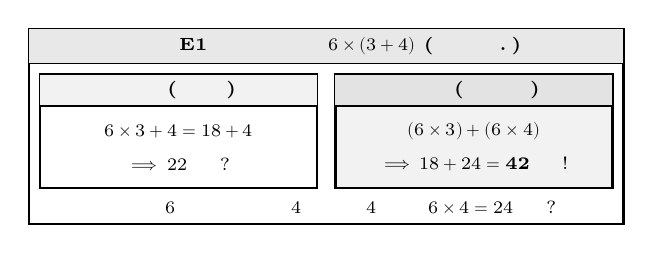
\begin{tikzpicture}[x=1cm, y=1cm, every node/.style={font=\fontsize{6.4pt}{8.4pt}\selectfont, text=black}]
  \draw[black, line width=0.9pt] (0,0) rectangle (7.55,2.48);
  \fill[gray!18] (0,2.04) rectangle (7.55,2.48);
  \draw[black, line width=0.6pt] (0,2.04) -- (7.55,2.04);
  \node at (3.775,2.26) {\textbf{បេសកកម្ម \en{E1}៖ អន្ទាក់ការបំបែកផលគុណ $6 \times (3 + 4)$ (ឧទាហរណ៍ ៣ ទំ.៨)}};

  % Left: Student A
  \draw[black, line width=0.8pt] (0.14,0.46) rectangle (3.66,1.90);
  \fill[gray!10] (0.14,1.50) rectangle (3.66,1.90);
  \draw[black, line width=0.5pt] (0.14,1.50) -- (3.66,1.50);
  \node at (1.90,1.70) {\textbf{សិស្ស ក (គុណតែតួទី១)}};
  \node at (1.90,1.18) {$6 \times 3 + 4 = 18 + 4$};
  \node at (1.90,0.76) {$\implies 22\text{ ការ៉ូ}$?};

  % Right: Student B
  \draw[black, line width=0.95pt, fill=gray!10] (3.89,0.46) rectangle (7.41,1.90);
  \fill[gray!22] (3.89,1.50) rectangle (7.41,1.90);
  \draw[black, line width=0.55pt] (3.89,1.50) -- (7.41,1.50);
  \node at (5.65,1.70) {\textbf{សិស្ស ខ (គុណទាំង ២ តួ)}};
  \node at (5.65,1.18) {$(6 \times 3) + (6 \times 4)$};
  \node at (5.65,0.76) {$\implies 18 + 24 = \mathbf{42}\text{ \textbf{ការ៉ូ}}$!};

  \node at (3.775,0.21) {\textbf{សំណួរ៖} បើមាន $6$ ជួរដេក តើការ៉ូប្រផេះ $4$ ជួរឈរមានតែ $4$ ការ៉ូ ឬ $6\times 4 = 24$ ការ៉ូ?};
\end{tikzpicture}}

% ២. E2 Explore: រូបក្រឡាការ៉ូបំបែក 6 x (3 + 4) = 18 + 24 (ឧទាហរណ៍ ៣ ទំ.៨)
\newcommand{\figArrayWNOneFour}{%
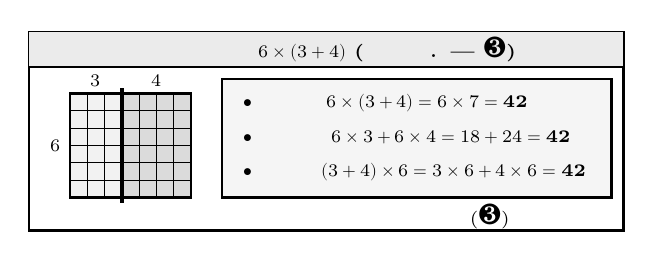
\begin{tikzpicture}[x=1cm, y=1cm, every node/.style={font=\fontsize{6.4pt}{8.4pt}\selectfont, text=black}]
  \draw[black, line width=0.9pt] (0,0) rectangle (7.55,2.52);
  \fill[gray!16] (0,2.08) rectangle (7.55,2.52);
  \draw[black, line width=0.6pt] (0,2.08) -- (7.55,2.08);
  \node at (3.775,2.30) {\textbf{គំរូក្រឡាការ៉ូបំបែកផ្ទៃ $6 \times (3 + 4)$ (ឧទាហរណ៍ ៣ ទំ.៨ — \cnum{3})}};

  % Grid 7 cols x 6 rows scaled by 0.22cm
  \begin{scope}[shift={(0.52,0.42)}, scale=0.22]
    \fill[gray!10] (0,0) rectangle (3,6);
    \fill[gray!28] (3,0) rectangle (7,6);
    \draw[black, line width=0.35pt] (0,0) grid (7,6);
    \draw[black, line width=0.85pt] (0,0) rectangle (7,6);
    \draw[black, line width=1.35pt] (3,-0.3) -- (3,6.3);
    \node at (-0.85,3) {$6$};
    \node at (1.5,6.75) {$3$};
    \node at (5.0,6.75) {$4$};
  \end{scope}

  % Explanation box on right
  \draw[black, line width=0.85pt, fill=gray!8] (2.45,0.42) rectangle (7.40,1.92);
  \node[anchor=west] at (2.60,1.62) {$\bullet$ សរុបទាំងមូល៖ $6 \times (3 + 4) = 6 \times 7 = \mathbf{42}$ ការ៉ូ};
  \node[anchor=west] at (2.60,1.18) {$\bullet$ តាម ២ ប្លុក៖ $6\times 3 + 6\times 4 = 18 + 24 = \mathbf{42}$};
  \node[anchor=west] at (2.60,0.74) {$\bullet$ គុណពីស្ដាំ៖ $(3 + 4)\times 6 = 3\times 6 + 4\times 6 = \mathbf{42}$};

  \node at (3.775,0.18) {សន្និដ្ឋាន៖ កត្តាខាងក្រៅត្រូវគុណនឹង\textbf{គ្រប់តួទាំងអស់}នៅក្នុងវង់ក្រចក (\cnum{3})};
\end{tikzpicture}}

% ៣. E3 Explain: តារាងប្រៀបធៀបលក្ខណៈវិធីបូក និងវិធីគុណ (ទំ.៦-៨)
\newcommand{\figPropsWNOneFour}{%
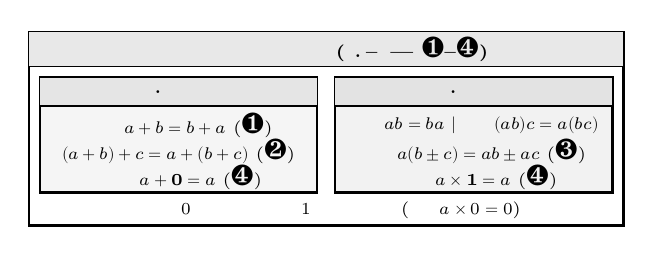
\begin{tikzpicture}[x=1cm, y=1cm, every node/.style={font=\fontsize{6.1pt}{8.1pt}\selectfont, text=black}]
  \draw[black, line width=0.9pt] (0,0) rectangle (7.55,2.46);
  \fill[gray!18] (0,2.02) rectangle (7.55,2.46);
  \draw[black, line width=0.6pt] (0,2.02) -- (7.55,2.02);
  \node at (3.775,2.24) {\textbf{ប្រៀបធៀបលក្ខណៈនៃវិធីបូក និងវិធីគុណ (ទំ.៦--៨ — \cnum{1}--\cnum{4})}};

  % Left: Addition
  \draw[black, line width=0.85pt, fill=gray!8] (0.14,0.42) rectangle (3.66,1.88);
  \fill[gray!20] (0.14,1.52) rectangle (3.66,1.88);
  \draw[black, line width=0.5pt] (0.14,1.52) -- (3.66,1.52);
  \node at (1.90,1.70) {\textbf{៥.១ វិធីបូក}};
  \node at (1.90,1.28) {ត្រឡប់៖ $a + b = b + a$ (\cnum{1})};
  \node at (1.90,0.95) {$(a+b)+c = a+(b+c)$ (\cnum{2})};
  \node at (1.90,0.62) {ធាតុណឺត៖ $a + \mathbf{0} = a$ (\cnum{4})};

  % Right: Multiplication
  \draw[black, line width=0.85pt, fill=gray!10] (3.89,0.42) rectangle (7.41,1.88);
  \fill[gray!22] (3.89,1.52) rectangle (7.41,1.88);
  \draw[black, line width=0.5pt] (3.89,1.52) -- (7.41,1.52);
  \node at (5.65,1.70) {\textbf{៥.២ វិធីគុណ}};
  \node at (5.65,1.28) {ត្រឡប់ $ab=ba$ $\mid$ ផ្ដុំ $(ab)c=a(bc)$};
  \node at (5.65,0.95) {បំបែក៖ $a(b\pm c) = ab \pm ac$ (\cnum{3})};
  \node at (5.65,0.62) {ធាតុណឺត៖ $a \times \mathbf{1} = a$ (\cnum{4})};

  \node at (3.775,0.20) {\textbf{ប្រយ័ត្ន៖} $0$ ជាធាតុណឺតវិធីបូក រីឯ $1$ ជាធាតុណឺតវិធីគុណ (ចំណែក $a\times 0 = 0$)};
\end{tikzpicture}}

% ៤. E4 Elaborate: លំហាត់គំរូចានកូនឃ្លី (ទំ.៨) និងប្រតិបត្តិផ្លែក្រូច (ទំ.៩)
\newcommand{\figMarbleWNOneFour}{%
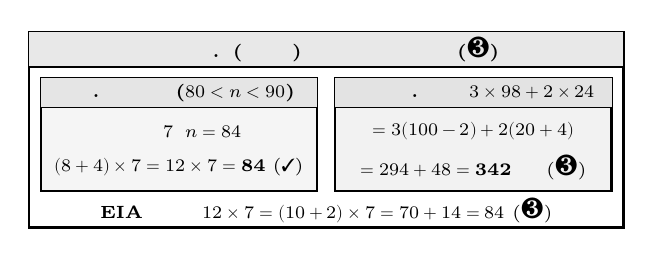
\begin{tikzpicture}[x=1cm, y=1cm, every node/.style={font=\fontsize{6.4pt}{8.4pt}\selectfont, text=black}]
  \draw[black, line width=0.9pt] (0,0) rectangle (7.55,2.48);
  \fill[gray!18] (0,2.04) rectangle (7.55,2.48);
  \draw[black, line width=0.6pt] (0,2.04) -- (7.55,2.04);
  \node at (3.775,2.26) {\textbf{លំហាត់គំរូទំ.៨ (ចានកូនឃ្លី) និងការគណនារហ័សតាមលក្ខណៈបំបែក (\cnum{3})}};

  % Left: Marble puzzle p.8
  \draw[black, line width=0.8pt, fill=gray!8] (0.15,0.46) rectangle (3.66,1.90);
  \fill[gray!20] (0.15,1.52) rectangle (3.66,1.90);
  \draw[black, line width=0.5pt] (0.15,1.52) -- (3.66,1.52);
  \node at (1.905,1.71) {\textbf{គំរូទំ.៨៖ ចានកូនឃ្លី ($80<n<90$)}};
  \node at (1.905,1.22) {ពហុគុណនៃ $7$៖ $n = 84$};
  \node at (1.905,0.76) {$(8+4)\times 7 = 12\times 7 = \mathbf{84}$ (\ding{51})};

  % Right: Mental math orange crates p.9
  \draw[black, line width=0.85pt, fill=gray!10] (3.89,0.46) rectangle (7.40,1.90);
  \fill[gray!22] (3.89,1.52) rectangle (7.40,1.90);
  \draw[black, line width=0.5pt] (3.89,1.52) -- (7.40,1.52);
  \node at (5.645,1.71) {\textbf{ប្រតិបត្តិទំ.៩៖ ក្រូច $3\times 98 + 2\times 24$}};
  \node at (5.645,1.22) {$= 3(100-2) + 2(20+4)$};
  \node at (5.645,0.76) {$= 294 + 48 = \mathbf{342\text{ \textbf{ផ្លែ}}}$ (\cnum{3})};

  \node at (3.775,0.22) {\textbf{\en{EIA}៖} គណនារហ័ស $12 \times 7 = (10+2)\times 7 = 70 + 14 = 84$ (\cnum{3})};
\end{tikzpicture}}

% ៥. E5 Evaluate: សំណួរវិនិច្ឆ័យ A-D លើលក្ខណៈបំបែក 8 x (10 + 5)
\newcommand{\figExitWNOneFour}{%
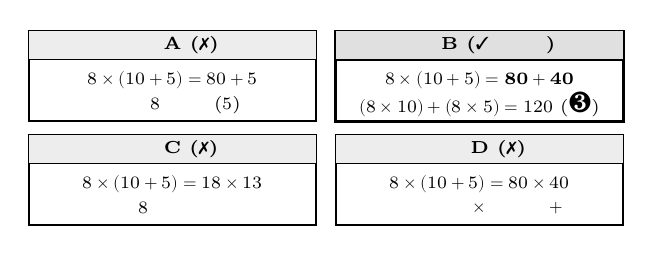
\begin{tikzpicture}[x=1cm, y=1cm, every node/.style={font=\fontsize{6.3pt}{8.2pt}\selectfont, text=black}]
  % Choice A
  \draw[black, line width=0.8pt] (0,1.32) rectangle (3.65,2.46);
  \fill[gray!14] (0,2.10) rectangle (3.65,2.46);
  \draw[black, line width=0.5pt] (0,2.10) -- (3.65,2.10);
  \node at (1.825,2.28) {\textbf{ជម្រើស \en{A} (\ding{55})}};
  \node at (1.825,1.84) {$8 \times (10 + 5) = 80 + 5$};
  \node at (1.825,1.53) {ភ្លេចគុណ $8$ នឹងតួទី២ ($5$)};

  % Choice B (Correct)
  \draw[black, line width=1.05pt] (3.90,1.32) rectangle (7.55,2.46);
  \fill[gray!24] (3.90,2.10) rectangle (7.55,2.46);
  \draw[black, line width=0.6pt] (3.90,2.10) -- (7.55,2.10);
  \node at (5.725,2.28) {\textbf{ជម្រើស \en{B} (\ding{51} ត្រឹមត្រូវ)}};
  \node at (5.725,1.84) {$8 \times (10 + 5) = \mathbf{80 + 40}$};
  \node at (5.725,1.53) {$(8\times 10)+(8\times 5) = 120$ (\cnum{3})};

  % Choice C
  \draw[black, line width=0.8pt] (0,0) rectangle (3.65,1.14);
  \fill[gray!14] (0,0.78) rectangle (3.65,1.14);
  \draw[black, line width=0.5pt] (0,0.78) -- (3.65,0.78);
  \node at (1.825,0.96) {\textbf{ជម្រើស \en{C} (\ding{55})}};
  \node at (1.825,0.52) {$8 \times (10 + 5) = 18 \times 13$};
  \node at (1.825,0.22) {ច្រឡំបូក $8$ ជាមួយតួក្នុងវង់ក្រចក};

  % Choice D
  \draw[black, line width=0.8pt] (3.90,0) rectangle (7.55,1.14);
  \fill[gray!14] (3.90,0.78) rectangle (7.55,1.14);
  \draw[black, line width=0.5pt] (3.90,0.78) -- (7.55,0.78);
  \node at (5.725,0.96) {\textbf{ជម្រើស \en{D} (\ding{55})}};
  \node at (5.725,0.52) {$8 \times (10 + 5) = 80 \times 40$};
  \node at (5.725,0.22) {ច្រឡំដាក់សញ្ញា $\times$ ជំនួសសញ្ញា $+$};
\end{tikzpicture}}

\begin{document}
\fontsize{10pt}{15.2pt}\selectfont

% ============================================================================
% ក្បាលរដ្ឋបាល (Administrative Header — តាមគំរូ ls_plan.tex)
% ============================================================================
{\centering
  {\muol\fontsize{11pt}{16pt}\selectfont ព្រះរាជាណាចក្រកម្ពុជា\par}
  {\muol\fontsize{11pt}{16pt}\selectfont ជាតិ សាសនា ព្រះមហាក្សត្រ\par}
  \vspace{-3pt}{\khmflourish\par}
}

\vspace{1pt}
{\muol\fontsize{10pt}{15.5pt}\selectfont
មន្ទីរអប់រំ យុវជន និងកីឡា ខេត្តកំពង់ធំ\par
ការិយាល័យអប់រំ យុវជន និងកីឡា ស្រុកកំពង់ស្វាយ\par
អនុវិទ្យាល័យព្រះក្រសាំង\par}

\vspace{2pt}
{\centering{\muol\fontsize{11.5pt}{17pt}\selectfont កិច្ចតែងការបង្រៀន\par}}
\vspace{2pt}

% --- ព័ត៌មានទូទៅ ---
{\hspace*{2.8cm}\renewcommand{\arraystretch}{1.08}
\begin{tabular}{@{}l@{\hspace{0.35cm}}p{2.9cm}@{\hspace{0.15cm}}c@{\hspace{0.25cm}}l@{}}
  - & មុខវិជ្ជា & : & គណិតវិទ្យា ថ្នាក់ទី៧ (ពីជគណិត) \\
  - & ចំណងជើងមេរៀន & : & មេរៀនទី១៖ ចំនួនគត់ \\
  - & ចំណងជើងរង & : & ៥. លក្ខណៈនៃប្រមាណវិធីបូកនិងគុណ (ទំ.៦--៩) \\
  - & រយៈពេល & : & ១ ម៉ោងសិក្សា (៥០ នាទី) \\
  - & បង្រៀនដោយ & : & ហុក ប៊ុនថែន \\
  - & កាលបរិច្ឆេទ & : & ថ្ងៃសុក្រ ទី៦ ខែវិច្ឆិកា ឆ្នាំ២០២៦ \\
\end{tabular}\par}

\vspace{2pt}

% --- I. វត្ថុបំណង ---
{\muol\fontsize{10pt}{15.5pt}\selectfont \enbf{I.} វត្ថុបំណង\par}
\vspace{1pt}
{\renewcommand{\arraystretch}{1.10}
\begin{tabular}{@{}p{0.55cm}@{}p{2.35cm}@{\hspace{0.15cm}}c@{\hspace{0.25cm}}p{14.95cm}@{}}
  \hfill\wcirc\hspace{0.2cm} & វិជ្ជាសម្បទា & : & សិស្សប្រាប់បានពីលក្ខណៈត្រឡប់ លក្ខណៈផ្ដុំ និងធាតុណឺតនៃវិធីបូក ($0$) និងវិធីគុណ ($1$) ព្រមទាំងលក្ខណៈបំបែកនៃវិធីគុណចំពោះវិធីបូកនិងវិធីដក ($a(b\pm c)=ab\pm ac$) បានត្រឹមត្រូវ ។ \\
  \hfill\wcirc\hspace{0.2cm} & បំណិនសម្បទា & : & សិស្សប្រើលក្ខណៈត្រឡប់ ផ្ដុំ និងលក្ខណៈបំបែកដើម្បីគណនារហ័ស និងដោះស្រាយចំណោទក្នុងសៀវភៅគោល (ចានកូនឃ្លីទំ.៨ និងកេះផ្លែក្រូចទំ.៩) លើសន្លឹកកិច្ចការបានត្រឹមត្រូវ ។ \\
  \hfill\wcirc\hspace{0.2cm} & ចរិយាសម្បទា & : & សិស្សមានភាពរហ័សរហួនក្នុងការជ្រើសរើសលក្ខណៈប្រមាណវិធីមកគណនាកាត់បន្ថយជំហាន មានទម្លាប់ផ្ទៀងផ្ទាត់គ្រប់តួក្នុងវង់ក្រចក និងសហការគ្នាជាក្រុម ។ \\
\end{tabular}\par}

\vspace{2pt}

% --- II. សម្ភារៈឧបទេស ---
{\muol\fontsize{10pt}{15.5pt}\selectfont \enbf{II.} សម្ភារៈឧបទេស\par}
\vspace{1pt}
\hspace*{0.55cm}$\bullet$\ សៀវភៅសិក្សាគោលថ្នាក់ទី៧ (ទំ.៦--៩ និងទំ.១៤) ក្ដារខៀន ដីស/ហ្វឺត បន្ទាត់ត្រង់ និង\textbf{សន្លឹកកិច្ចការសិស្សបំពេញចន្លោះ ស-ខ្មៅ} (កូដ \en{WN14} ទំព័រ ១--២ សម្រាប់សិស្ស និងទំព័រ ៣ ប្លង់ក្ដារខៀន/ចម្លើយគ្រូ — គ្មានប្រើ \en{LCD})\par

\vspace{2pt}

% --- III. វិធីសាស្រ្តបង្រៀន ---
{\muol\fontsize{10pt}{15.5pt}\selectfont \enbf{III.} វិធីសាស្រ្តបង្រៀន\par}
\vspace{1pt}
{\renewcommand{\arraystretch}{1.08}
\begin{tabular}{@{}p{0.55cm}@{}p{2.35cm}@{\hspace{0.15cm}}c@{\hspace{0.25cm}}p{14.95cm}@{}}
  \hfill$\bullet$\hspace{0.2cm} & គោលវិធី & : & សិស្សមជ្ឈមណ្ឌល (សន្លឹកកិច្ចការបំពេញចន្លោះជាគោល + ការពិភាក្សាជាក្រុមតូច ៣ នាក់) \\
  \hfill$\bullet$\hspace{0.2cm} & យុទ្ធវិធីបង្រៀន & : & គំរូស្ថាបនានិយម \en{5Es} រួមបញ្ចូល \textbf{គំរូក្រឡាការ៉ូបំបែកផ្ទៃ (\en{Split Rectangular Array})} និង \textbf{តារាងប្រៀបធៀបលក្ខណៈទន្ទឹមគ្នា (\en{Contrasting Properties Matrix})} \\
\end{tabular}\par}

\vspace{2pt}

% --- IV. ដំណើរការបង្រៀន ---
{\muol\fontsize{10pt}{15.5pt}\selectfont \enbf{IV.} ដំណើរការបង្រៀន\par}

{\renewcommand{\arraystretch}{1.15}
\begin{longtable}{|L{5.50cm}|L{7.90cm}|L{4.80cm}|}
\hline
\multicolumn{1}{|c|}{\cellcolor{headgray}\muol សកម្មភាពគ្រូ} &
\multicolumn{1}{c|}{\cellcolor{headgray}\muol ខ្លឹមសារមេរៀន} &
\multicolumn{1}{c|}{\cellcolor{headgray}\muol សកម្មភាពសិស្ស} \\
\hline
\endfirsthead

\hline
\multicolumn{1}{|c|}{\cellcolor{headgray}\muol សកម្មភាពគ្រូ} &
\multicolumn{1}{c|}{\cellcolor{headgray}\muol ខ្លឹមសារមេរៀន} &
\multicolumn{1}{c|}{\cellcolor{headgray}\muol សកម្មភាពសិស្ស} \\
\hline
\endhead

% ==================== ជំហានទី១ (2min) ====================
\stepheader{ជំហានទី១ \enbf{(}រដ្ឋបាលថ្នាក់\enbf{)}}
$\bullet$ ពិនិត្យវត្តមាន អនាម័យ និងសណ្ដាប់ធ្នាប់ថ្នាក់រៀន \par
$\bullet$ រៀបចំក្រុមតូច ៣ នាក់តាមតុ និងចែក\textbf{សន្លឹកកិច្ចការសិស្ស (\en{WN14} ទំព័រ ១–២)}
&
$\bullet$ រដ្ឋបាលថ្នាក់ អនាម័យ និងវិន័យសិក្សា \par
$\bullet$ ចែកសន្លឹកកិច្ចការម្នាក់ ១ សន្លឹក សម្រាប់បំពេញតាមដំណាក់កាល \en{E1--E5}
&
$\circ$ ប្រធានថ្នាក់រាយការណ៍វត្តមានសិស្ស \par
$\circ$ ទទួលសន្លឹកកិច្ចការ សរសេរឈ្មោះ និងអង្គុយតាមក្រុម ៣ នាក់ \\
\hline

% ==================== ជំហានទី២ (9min: កំណែ <=3m + រំលឹក 3m + E1 3m) ====================
\stepheader{ជំហានទី២ \enbf{(}កិច្ចការផ្ទះ \enbf{+} ទំនាក់ទំនងមេរៀនថ្មី\enbf{)}}
\ditem \textbf{កំណែកិច្ចការផ្ទះ ($\le\text{\enbf{3\,min}}$)} \par
$\bullet$ ហៅសិស្ស ២ នាក់ឡើងកែលំហាត់ទំ.១៤ លេខ ៤ និង លេខ ៥ លើក្ដារខៀនផ្នែកឆ្វេង
&
{\centering\redsub{កំណែកិច្ចការផ្ទះមេរៀនមុន (ទំ.១៤ លេខ ៤ និង លេខ ៥)}\par}
$\bullet$ \textbf{លេខ ៤៖} មៀននៅសល់ $5\times 10 - 8 = 42$ ផ្លែ $\implies$ ម្នាក់ៗបាន $42 \div 6 = \mathbf{7}$ ផ្លែ \par
$\bullet$ \textbf{លេខ ៥៖} សិស្សសរុប $76 \div 2 = 38$ នាក់ $\implies$ សិស្សស្រី $38 - 18 = \mathbf{20}$ នាក់
&
$\circ$ ផ្ទៀងចម្លើយ ($7$ ផ្លែ និង $20$ នាក់) និងកែចូលសៀវភៅ \\[3pt]

\ditem \textbf{រំលឹកមេរៀនទាក់ទង (\enbf{3min})} \par
$\bullet$ សួរ៖ «បើគេរៀបការ៉ូជា $3$ ជួរដេក ហើយ ១ ជួរមាន $4$ ការ៉ូ តើរាប់តាមជួរដេក និងជួរឈរឃើញស្មើគ្នាដែរឬទេ?»
&
{\centering\redsub{រំលឹកផលគុណតាមក្រឡាការ៉ូចតុកោណកែង}\par}
$\bullet$ រាប់តាមជួរដេក៖ $3 \times 4 = 12$ ការ៉ូ $\mid$ រាប់តាមជួរឈរ៖ $4 \times 3 = 12$ ការ៉ូ
&
$\circ$ ឆ្លើយ៖ «ស្មើគ្នា គឺ $12$ ការ៉ូដូចគ្នា!» \\[3pt]

$\bullet$ សួរបន្ត៖ «ចុះបូកថែម $0$ និងគុណនឹង $1$ តើតម្លៃចំនួនដើមប្រែប្រួលឬទេ?»
&
$\bullet$ $14 + 0 = 14$ និង $14 \times 1 = 14$ (តម្លៃដើមមិនប្រែប្រួលទេ រីឯ $14 \times 0 = 0$)
&
$\circ$ កត់សម្គាល់ភាពខុសគ្នារវាង $+0$, $\times 1$ និង $\times 0$ \\[3pt]

\fiveE{E1 - Engage (3min)} \timenote{(កុំទាន់ផ្ដល់ចម្លើយ)} \par
\ditem \textbf{បេសកកម្មអន្ទាក់ការបំបែក $6 \times (3 + 4)$ (សន្លឹកកិច្ចការ \en{E1})} \par
$\bullet$ ឱ្យសិស្សអានប្រអប់ \en{E1} (ឧទាហរណ៍ ៣ ទំ.៨) ហើយជ្រើសរើសរវាង\textbf{សិស្ស ក} និង\textbf{សិស្ស ខ}
&
\redsub{បេសកកម្ម \en{E1}៖ គណនាចំនួនការ៉ូសរុប $6 \times (3 + 4)$ (ទំ.៨)} \par
$\bullet$ \textbf{សិស្ស ក} បំបែកជា $6 \times 3 + 4 = 22$ ការ៉ូ \par
$\bullet$ \textbf{សិស្ស ខ} បំបែកជា $(6 \times 3) + (6 \times 4) = 42$ ការ៉ូ ។ តើអ្នកណាត្រឹមត្រូវ?
&
$\circ$ ពិភាក្សាជាគូ និងគូស \ding{51} ក្នុងប្រអប់ \en{E1} លើសន្លឹកកិច្ចការ \\[3pt]

&
\cfig{\figEngageWNOneFour}
& \\
\hline

% ==================== ជំហានទី៣ (17min: E2 11m + E3 6m) ====================
\stepheader{ជំហានទី៣ \enbf{(}ខ្លឹមសារមេរៀនថ្មី\enbf{)}}
\fiveE{E2 - Explore (11min)} \par
$\bullet$ សរសេរចំណងជើងរង \textbf{៥. លក្ខណៈនៃប្រមាណវិធី} លើក្ដារខៀន \par
\ditem \textbf{សកម្មភាព ១៖ លក្ខណៈត្រឡប់ ផ្ដុំ និងធាតុណឺត (ទំ.៦--៨, \enbf{5min}, \en{E2-A})} \par
$\bullet$ ឱ្យសិស្សបំពេញឧទាហរណ៍ ១--៣ នៃវិធីបូក (ទំ.៦--៧) និងឧទាហរណ៍ ១, ២, ៤ នៃវិធីគុណលើ \en{E2-A}
&
៥. លក្ខណៈនៃប្រមាណវិធី \par
$\bullet$ \textbf{៥.១ វិធីបូក (ទំ.៦--៧)៖} $4+5 = 5+4 = \mathbf{9}$ (ត្រឡប់); $(2+3)+5 = 2+(3+5) = \mathbf{10}$ (ផ្ដុំ); $1+0 = 0+1 = \mathbf{1}$ ($0$ ជាធាតុណឺត) \par
$\bullet$ \textbf{៥.២ វិធីគុណ (ទំ.៧--៨)៖} $7\times 5 = 5\times 7 = \mathbf{35}$; $5\times(3\times 4) = 4\times(3\times 5) = \mathbf{60}$; $1\times 14 = 14\times 1 = \mathbf{14}$ ($1$ ជាធាតុណឺត)
&
$\circ$ គណនានិងប្រៀបធៀបលទ្ធផលទាំងសងខាងលើ \en{E2-A} \\[3pt]

\ditem \textbf{សកម្មភាព ២៖ រូបក្រឡាការ៉ូបំបែកនៃវិធីគុណ (ទំ.៨, \enbf{6min}, \en{E2-B})} \par
$\bullet$ ឱ្យសិស្សពិនិត្យរូបក្រឡាការ៉ូ $6$ ជួរដេក $\times (3+4)$ ជួរឈរ លើ \en{E2-B} រួចគណនាតាម ២ របៀប
&
$\bullet$ \textbf{ឧទាហរណ៍ ៣ (ទំ.៨ — លក្ខណៈបំបែកនៃវិធីគុណចំពោះវិធីបូក)៖} \par
\hspace*{0.2cm}របៀបទី១ (រាប់សរុប)៖ $6 \times (3 + 4) = 6 \times 7 = \mathbf{42}$ ការ៉ូ \par
\hspace*{0.2cm}របៀបទី២ (បំបែក ២ ប្លុក)៖ $(6 \times 3) + (6 \times 4) = 18 + 24 = \mathbf{42}$ ការ៉ូ
&
$\circ$ រាប់ក្រឡាការ៉ូស ($18$) និងប្រផេះ ($24$) ឃើញសរុប $42$ ស្មើគ្នា \\[3pt]

$\bullet$ ឱ្យសិស្សសាកល្បងគុណពីខាងស្ដាំ $(3+4)\times 6$ និងចំពោះវិធីដក $6\times(7-3)$
&
$\bullet$ គុណពីខាងស្ដាំ៖ $(3 + 4) \times 6 = (3 \times 6) + (4 \times 6) = 18 + 24 = \mathbf{42}$ \par
$\bullet$ ចំពោះវិធីដក៖ $6 \times (7 - 3) = (6 \times 7) - (6 \times 3) = 42 - 18 = \mathbf{24}$
&
$\circ$ សន្និដ្ឋានថាលក្ខណៈបំបែកប្រើបានទាំងវិធីបូក និងវិធីដក \\[3pt]

&
\cfig{\figArrayWNOneFour}
& \\[3pt]

% --- E3 Explain (6min) ---
\fiveE{E3 - Explain (6min)} \par
$\bullet$ ដឹកនាំសិស្សសង្ខេបរូបមន្តជាទូទៅនៃវិធីបូកនិងវិធីគុណ (ទំ.៦--៨) លើ \en{E3}
&
$\bullet$ \textbf{រូបមន្តជាទូទៅ ចំពោះគ្រប់ចំនួនគត់ $a, b, c$ (ទំ.៦--៨)៖} \par
\hspace*{0.15cm}១) វិធីបូក៖ $a+b=b+a$; $(a+b)+c=a+(b+c)$; ធាតុណឺតគឺ \graybox{$0$} ($a+0=a$) \par
\hspace*{0.15cm}២) វិធីគុណ៖ $ab=ba$; $(ab)c=a(bc)$; ធាតុណឺតគឺ \graybox{$1$} ($a\times 1=a$)
&
$\circ$ បំពេញប្រអប់ធាតុណឺត $0$ និង $1$ លើសន្លឹកកិច្ចការ \en{E3} \\[3pt]

$\bullet$ ឱ្យសិស្សសរសេររូបមន្តលក្ខណៈបំបែក និងភ្ជាប់\textbf{ធនាគារហេតុផល \cnum{1}--\cnum{2}}
&
\hspace*{0.15cm}៣) លក្ខណៈបំបែក៖ \graybox{$a(b + c) = ab + ac$} និង \graybox{$a(b - c) = ab - ac$} \par
\cnum{1} \textbf{លក្ខណៈត្រឡប់៖} ប្ដូរទីតាំងតួបូក ឬកត្តាគុណ ($a+b=b+a, \ ab=ba$) \par
\cnum{2} \textbf{លក្ខណៈផ្ដុំ៖} ផ្ដុំគូតួដែលបូក ឬគុណចេញលេខគត់ដប់/រយ ($25\times 4 = 100$)
&
$\circ$ បំពេញរូបមន្តបំបែក និងផ្ទៀងលេខកូដ \cnum{1}--\cnum{2} \\[3pt]

$\bullet$ ភ្ជាប់\textbf{ធនាគារហេតុផល \cnum{3}--\cnum{4}} (បំបែក និងធាតុណឺត) លើក្ដារខៀន
&
\cnum{3} \textbf{លក្ខណៈបំបែក៖} $a(b\pm c) = ab \pm ac$ (ឬទាញកត្តារួម $ab \pm ac = a(b\pm c)$) \par
\cnum{4} \textbf{ធាតុណឺត៖} $0$ ចំពោះវិធីបូក ($a+0=a$); $1$ ចំពោះវិធីគុណ ($a\times 1=a$)
&
$\circ$ ផ្ទៀងលេខកូដ \cnum{3}--\cnum{4} លើសន្លឹកកិច្ចការ \\[3pt]

&
\cfig{\figPropsWNOneFour}
& \\
\hline

% ==================== ជំហានទី៤ (20min: E4 10m + E5 10m) ====================
\stepheader{ជំហានទី៤ \enbf{(}ពង្រីកចំណេះដឹង\enbf{)}}
\fiveE{E4 - Elaborate (10min)} \par
\ditem \textbf{លំហាត់គំរូ៖ ចំណោទចានកូនឃ្លី (សៀវភៅគោល ទំ.៨)} \par
$\bullet$ ឱ្យសិស្សអានប្រធានលំហាត់គំរូទំ.៨ និងកំណត់លក្ខខណ្ឌនៃចំនួនកូនឃ្លី $n$ លើ \en{E4}
&
{\muol លំហាត់គំរូ} \textbf{(ទំ.៨ — កូនឃ្លីច្រើនជាង $80$ តែតិចជាង $90$ ស្មើ $7$ ដងផលបូកតួលេខ)៖} \par
$\bullet$ \textbf{ជំហានទី១៖} តាង $n$ ជាចំនួនគ្រាប់ឃ្លី ដែល $80 < n < 90$ ហើយ $n$ ជាពហុគុណនៃ $7$
&
$\circ$ កំណត់ចន្លោះ $80 < n < 90$ និងពហុគុណនៃ $7$ (គឺ $84$) \\[3pt]

$\bullet$ ឱ្យសិស្សផ្ទៀងផ្ទាត់តម្លៃ $n = 81$ និង $n = 84$ តាមលក្ខខណ្ឌប្រធានលើ \en{E4}
&
$\bullet$ \textbf{ជំហានទី២៖} បើ $n=81 \implies (8+1)\times 7 = 63 \ne 81$ (\ding{55}) \par
\hspace*{0.2cm}បើ $n=84 \implies (8+4)\times 7 = 12\times 7 = \mathbf{84}$ (\ding{51}) ។ ដូច្នេះមានកូនឃ្លី \graybox{$84\text{ គ្រាប់}$}
&
$\circ$ ផ្ទៀងផ្ទាត់ឃើញ $n = 84$ គ្រាប់ពិតជាផ្ទៀងផ្ទាត់លក្ខខណ្ឌ \\[3pt]

&
\cfig{\figMarbleWNOneFour}
& \\[3pt]

$\bullet$ សួរសំណួរឆ្លុះបញ្ចាំង \textbf{\en{EIA Looking-Back} (1min)} លើការគណនា $12 \times 7$
&
\textbf{\en{EIA Looking-Back}៖} «តើយើងអាចគណនា $12 \times 7$ ក្នុងចិត្តដោយប្រើលក្ខណៈបំបែក (\cnum{3}) ដូចម្ដេច?» $\to 12\times 7 = (10 + 2)\times 7 = 70 + 14 = \mathbf{84}$!
&
$\circ$ បំបែក $12 = 10 + 2$ គណនាឃើញ $84$ យ៉ាងរហ័ស \\[3pt]

% --- E5 Evaluate (10min) ---
\fiveE{E5 - Evaluate (10min)} \par
\ditem \textbf{ប្រតិបត្តិជាក្រុមតូច ៣ នាក់ (4min, សន្លឹកកិច្ចការ \en{E5})} \par
$\bullet$ ឱ្យក្រុមសិស្សដោះស្រាយលំហាត់ប្រតិបត្តិទំ.៩ (ផ្លែក្រូច $3$ កេះធំ និង $2$ កេះតូច) ដោយប្រើលក្ខណៈបំបែក
&
{\muol លំហាត់ប្រតិបត្តិ} \textbf{(ទំ.៩ — ក្រូច $3$ កេះធំ $\times 98$ ផ្លែ និង $2$ កេះតូច $\times 24$ ផ្លែ)៖} \par
$\bullet$ កន្សោមសរុប៖ $3 \times 98 + 2 \times 24 = 3 \times (100 - 2) + 2 \times (20 + 4)$ \par
$\bullet$ តាម \cnum{3}៖ $= (300 - 6) + (40 + 8) = 294 + 48 = \graybox{$342\text{ ផ្លែ}$}$
&
$\circ$ បំបែក $98 = 100 - 2$ និង $24 = 20 + 4$ គណនាឃើញ $342$ ផ្លែ \\[3pt]

$\bullet$ ឱ្យក្រុមសិស្សផ្ទៀងផ្ទាត់និង\textbf{បិទបេសកកម្ម \en{E1} (2min)}
&
$\bullet$ \textbf{បិទបេសកកម្ម \en{E1}៖} \textbf{សិស្ស ខ} ត្រឹមត្រូវ! $6 \times (3 + 4) = 18 + 24 = \mathbf{42}$ ការ៉ូ (\cnum{3}) ព្រោះកត្តា $6$ ត្រូវគុណនឹងតួទាំងពីរក្នុងវង់ក្រចក ។
&
$\circ$ បិទបេសកកម្ម \en{E1} ឃើញសិស្ស ខ ត្រឹមត្រូវ ($42$ ការ៉ូ) \\[3pt]

\ditem \textbf{សំណួរវិនិច្ឆ័យ \en{A--D} និងសំបុត្រចេញ (4min)} \par
$\bullet$ សរសេរកន្សោម $8 \times (10 + 5)$ និងជម្រើស \en{A--D} លើក្ដារខៀន
&
{\centering\textbf{សំណួរវិនិច្ឆ័យ \en{A--D}៖ តើសមភាពមួយណាប្រើលក្ខណៈបំបែកបានត្រឹមត្រូវ?}\par}
&
$\circ$ ពិនិត្យជម្រើសនីមួយៗធៀបនឹងវិធាន \cnum{3} \\[3pt]

$\bullet$ ឱ្យសិស្សគូសរង្វង់ជម្រើសត្រូវលើសន្លឹកកិច្ចការ រួចលើកម្រាមដៃ ១--៤ ព្រមគ្នា
&
$\bullet$ វិភាគកំហុសក្នុងជម្រើស \en{A}, \en{C}, \en{D} តាមរូបមន្ត $a(b+c)=ab+ac$ (\cnum{3})
&
$\circ$ គូសរង្វង់លើសន្លឹកកិច្ចការ និងលើកម្រាមដៃ ២ (\textbf{ជម្រើស \en{B}}) \\[3pt]

&
\cfig{\figExitWNOneFour}
& \\[3pt]

$\bullet$ បញ្ជាក់ចម្លើយត្រូវ (\textbf{ជម្រើស \en{B}}) និងឱ្យបំពេញ\textbf{សំបុត្រចេញ ៦០ វិនាទី}
&
$\bullet$ \textbf{សំបុត្រចេញ៖} $27 \times 64 + 27 \times 36 = 27 \times (64 + 36) = 27 \times 100 = \mathbf{2\,700}$ (\cnum{3}) ។
&
$\circ$ ទាញកត្តារួម $27$ គណនាឃើញ $2\,700$ មុនបញ្ចប់ម៉ោង \\
\hline

% ==================== ជំហានទី៥ (<=2min) ====================
\stepheader{ជំហានទី៥ \enbf{(}កិច្ចការផ្ទះ \enbf{+} បណ្ដាំផ្ញើ\enbf{)}}
\timenote{ចំណាយពេលឱ្យតិចបំផុតកុំឱ្យលើស 2min} \par
$\bullet$ ណែនាំប្រអប់\textbf{កិច្ចការផ្ទះ}លើសន្លឹកកិច្ចការទំព័រ ២ (ទំ.១៤ លេខ ២ ក និងលំហាត់គណនារហ័ស)
&
{\centering{\muol កិច្ចការផ្ទះ} \textbf{(សៀវភៅគោល ទំ.១៤ លេខ ២ ក និងលំហាត់គណនារហ័ស)}\par} \par
$\bullet$ \textbf{១) ទំ.១៤ លេខ ២ ក៖} គណនាកន្សោម $40 \times 5 + 50 \times 6 - 7 \times 60$ ។ \par
$\bullet$ \textbf{២) គណនារហ័ស៖} ក. $25 \times 19 \times 4$ \quad ខ. $37 \times 64 + 37 \times 36$ \quad គ. $6 \times 99$ ។
&
$\circ$ គូសចំណាំកិច្ចការផ្ទះលើសន្លឹកកិច្ចការទំព័រ ២ \\[3pt]

$\bullet$ ផ្ដាំផ្ញើឱ្យធ្វើកិច្ចការផ្ទះ និងអានមុនចំណុច ៦ (ទំ.៩–១០)
&
$\bullet$ \textbf{បណ្ដាំផ្ញើ៖} អនុវត្តលក្ខណៈផ្ដុំនិងបំបែកក្នុងកិច្ចការផ្ទះ ហើយអានមុន \textbf{៦. លំដាប់នៃប្រមាណវិធីលើចំនួនគត់} (ទំ.៩–១០) ។
&
$\circ$ កត់ត្រាបណ្ដាំផ្ញើ ទុកសន្លឹកកិច្ចការក្នុងសៀវភៅ និងជម្រាបលាគ្រូ \\
\hline
\end{longtable}}

\vspace{6pt}
% --- ហត្ថលេខា (កាលបរិច្ឆេទត្រូវគ្នា ១០០% នឹងខាងលើ) ---
{\centering
\hspace*{5.2cm}\begin{minipage}{11.5cm}
  \centering
  ថ្ងៃសុក្រ ១១រោច ខែអស្សុជ ឆ្នាំមមី អដ្ឋស័ក ពុទ្ធសករាជ ២៥៧០\par
  កំពង់ស្វាយ, ថ្ងៃទី៦ ខែវិច្ឆិកា ឆ្នាំ២០២៦\par
  \vspace{2pt}
  {\muol គ្រូបង្រៀន\par}
  \vspace{32pt}
  \hfill{\muol ហុក ប៊ុនថែន}\hspace*{1.4cm}
\end{minipage}\par}

\end{document}
